\subsection{System Overview}
Through the system overview diagram, in figure \ref{fig:system_overview}, it is possible to identify the main modules of the system to be developed, and how they interact. We can divide the system into two subsystems: the local system, which represents a lamp post, and the monitoring device, which can monitor a network of lamp posts.

\begin{figure}[ht]
	\centering
	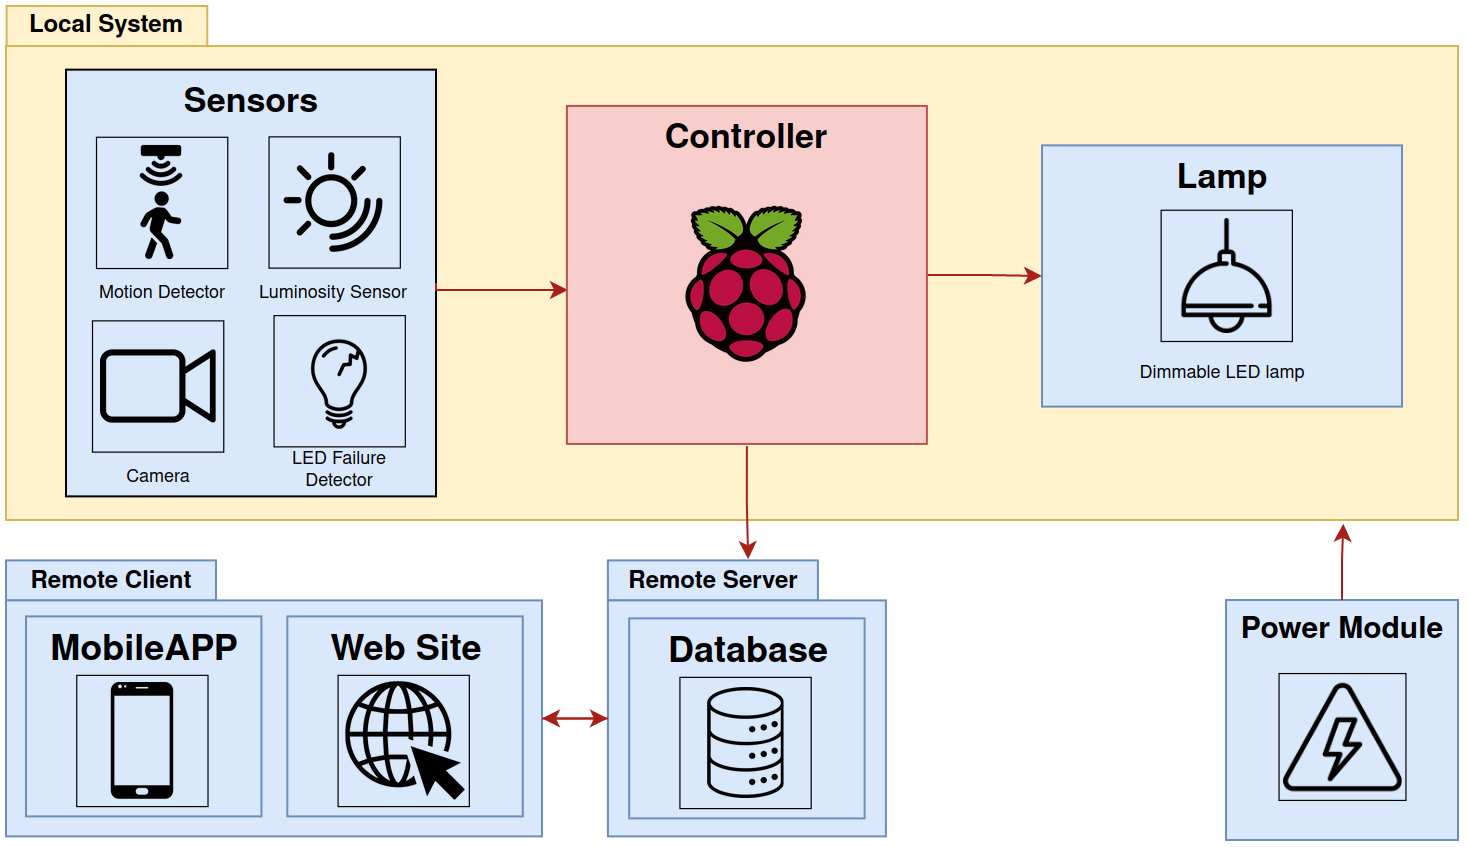
\includegraphics[width=1\textwidth]{system_overview}
	\caption{System Overview Diagram.}
	\label{fig:system_overview}
\end{figure}

The local system is composed of sensors, a controller and a lamp. Regarding the sensors, there will be a motion detector, to allow the detection of movement in the vicinity of the pole, a light sensor, to detect the light conditions of the pole’s surroundings, and a LED state sensor to know if the LED lamp is working. The controller, through sensors information, controls the luminosity of the lamp and communicates via wireless with the monitoring device. The monitoring device exchanges data with a database, recording all information relating to each local system. This information can also be viewed and managed by a mobile application, which can be accessed by a person responsible for the street lamp network. The monitoring device can also control a series of LEDs regarding network state. Knowing that the public lighting network is directly related to the electrical network, this will be used to power local systems, such as the monitoring device.

\subsection{System Requirements and Constraints}
In order for the system to have the desired performance, these requirements and constraints must be respected:

\subparagraph{Functional Requirements}
\begin{itemize}
	\item Sensors data acquisition				\item Motion detector
	\item Control of a street lamp
	\item Control a network of street poles		\item Wireless communication
	\item Access system information through a mobile application
\end{itemize}

\subparagraph{Non-Functional Requirements}
\begin{itemize}
	\item User friendly mobile application
	\item Ambient luminosity sensing
	\item Lower power consumption than actual street lights
	\item Soft Real-Time Embedded System
\end{itemize}

\subparagraph{Technical Constraints}
\begin{itemize}
	\item Buildroot
	\item C/C++ 
	\item Device Drivers
	\item Linux
	\item Raspberry Pi
	\item \ac{cps}
	\item Makefiles
	\item Pthreads
\end{itemize}

\subparagraph{Non-Technical Constraints}
\begin{itemize}
	\item Two members team
	\item Project deadline at the end of the semester
	\item Low budget
	
\end{itemize}

\section{System Architecture}
Using the system overview diagram information, one can describe the system in two different architectures. Hardware architecture, as how the hardware modules interfaces with itself, and what are the physical components of the system, and software architecture, which details how the information is processed among different software layers.

\subsection{Hardware Architecture}
In figure \ref{fig:hw_arch}, one can see the diagram that represents the physical connections of the system. The power of most system components will be the output of the DC/DC converter, powering the controller and its associated sensors. In order to power the lamp and at the same time control its brightness, a driver must be used, taking the controller output and system power as inputs. The Raspberry Pi, despite not belonging to the local system, is powered similarly to the controller, via a DC/DC converter. Furthermore, it communicates with the controller wirelessly through its wireless interface, with the controller's wireless communication module.

\begin{figure}[ht]
	\centering
	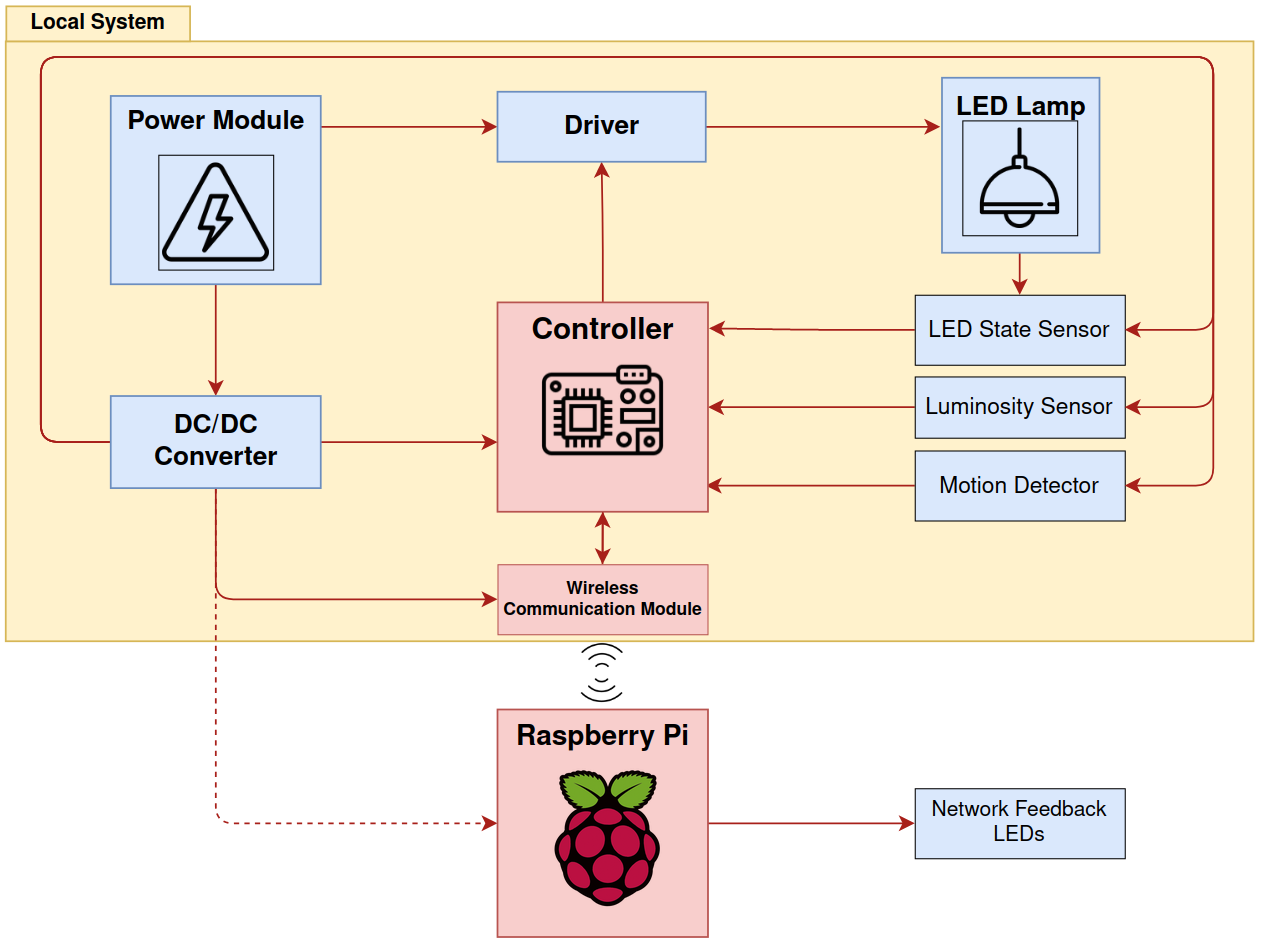
\includegraphics[width=1\textwidth]{hw_arch}
	\caption{Hardware Architecture Diagram.}
	\label{fig:hw_arch}
\end{figure}

\subsection{Software Architecture}
As seen previously, the system is divided into two subsystems: the local system and the monitoring system. Their software architectures are divided into three layers:

\begin{itemize}
	\item The Operating System layer, which is composed by the Operating System drivers and Board Support Packages;
	\item The Middleware layer, which includes software for abstracting the lower level layer packages. It works as a pipe since it links two applications, in different layers, so that data can be easily transmitted;
	\item The Application layer, where the core functionality of the program is built, with a resource for the API's in the lower level layers.
\end{itemize}

Regarding the local system, shown in figure \ref{fig:sw_arch_local}, the operating system layer is composed by the sensor drivers, such as the LED Failure Sensor, the Luminosity Sensor, the Motion Detector Sensor and also the Wireless Communication driver. As this system will acquire data from the environment through the mentioned sensors, at a low rate, and communicate this data to the monitoring device, multitasking will not be necessary, so this system will be bare metal, that is, it won’t have an operating system. In the middleware layer are the tools needed to acquire data from sensors and communicate wirelessly with the monitoring system. Finally, the communication between the different devices is managed in the application layer.

\begin{figure}[ht]
	\centering
	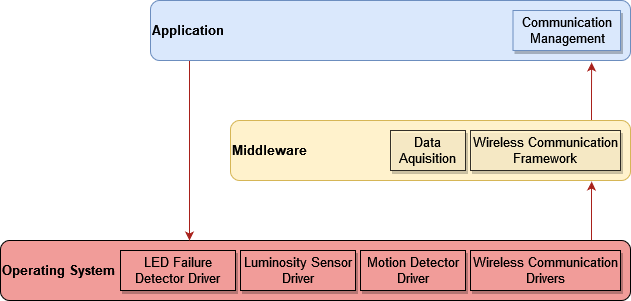
\includegraphics[width=1\textwidth]{sw_arch_local}
	\caption{Software Architecture Diagram - Local System.}
	\label{fig:sw_arch_local}
\end{figure}

Regarding the monitoring system, represented in figure \ref{fig:sw_arch_rasp}, the operating system layer is responsible for the network feedback LED drivers and for the wireless communication driver. This operating system will be a \ac{rtos}, due to the need to respond to events in a certain period of time and also multitasking. In the middleware layer, there will be the PThreads execution model, for multitasking, as well as the wireless communication and data acquisition frameworks. The application layer manages the system database, as well as the graphical user interface and all communications with local systems.

\begin{figure}[ht]
	\centering
	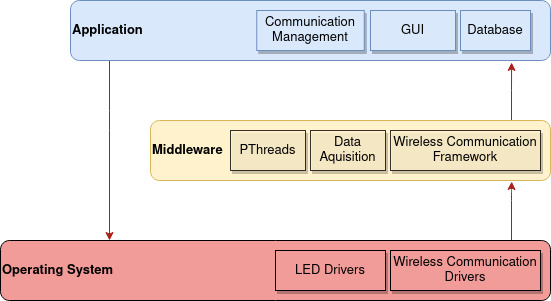
\includegraphics[width=1\textwidth]{sw_arch_rasp}
	\caption{Software Architecture Diagram - Monitoring System.}
	\label{fig:sw_arch_rasp}
\end{figure}
